\subsection{Geostationäre Projektion}
\label{sec:geostat}
In der geostationären Projektion wird die Erde aus der Perspektive eines geostationären Satelliten.
Vorteil:\newline \begin{itemize}
                  \item Wenn die Position des Satelliten bekannt ist, kann man dessen
                  Bilder als Hintergrund verwenden (siehe \ref{bilder})
                 \end{itemize}

Nachteil:\newline \begin{itemize}
                  \item Die andere Seite der Erde wird nicht dargestellt.\\
                  \item Entfernungen zwischen 2 Punkten werden auf Kreisbögen gemessen.\\
                  \item Der Satellit muss über dem Äquator sein.
                 \end{itemize}
\begin{figure}[hbtp]
\centering
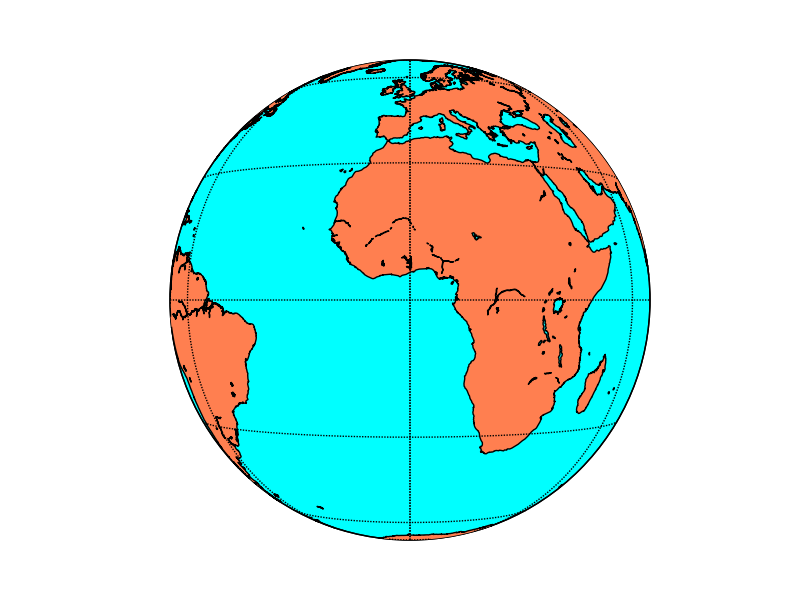
\includegraphics[scale=0.5,origin=c]{/Users/student/seminar/Kartendarstellungen/seminar/geos} \caption{Geostationäre Projektion}
\end{figure}
\newpage 